\section*{Einführung und Neurobiologische Grundlagen}%bis einschl. Kap 4
% Motivation
% Neurobiologische Grundlagen
% Geschichte
% Terminologie, Biologisches Neuron hier
% Bestandteilte neuronaler Netze
\begin{mytheo}{Neuronale Netze (NN)}
ssind informationsverarbeitende Systeme, die aus einer großen Anzahl einfacher Einheiten (Zellen, Neuronen)
bestehen, die sich Information in Form der Aktivierung der Zellen über
gerichtete Verbindungen (connections, links) zusenden.
\end{mytheo}
\noindent
Es  handelt sich hierbei um \textit{massiv parallele}, \textit{lernfähige} Systeme, die auch für sich
genommen als parallele Algorithmen interessant sind. 
Das wesentliche Element ist die Lernfähigkeit, die Fähigkeit, eine Aufgabe, wie etwa ein
Klassifikationsproblem, selbständig aus Trainingsbeispielen zu lernen, ohne dass
das neuronale Netz dazu explizit programmiert werden muss.\\
In verschiedenen Disziplinen spielen unterschiedliche
Gesichtspunkte neuronaler Netze eine Rolle:
\begin{itemize}[noitemsep]
\item (Neuro-)Biologie, Neurophysiologie und Medizin: NN, die in möglichst vieler
Hinsicht dem biologischen Vorbild entsprechen, so dass durch Simulation der
Modelle Rückschlüsse auf noch ungeklärte Eigenschaften des biologischen
Systems möglich werden. 
\item Psychologie: Modellierung, Simulation und Vorhersage psychologischer Phänomene des menschlichen Gehirns
\item Informatik: Eigenschaften neuronaler Netze als massiv parallele Algorithmen,
 ihre Lernfähigkeit und Effizienz. Sie werden dabei oft als ein zur
sogenannten (symbolischen) künstlichen Intelligenz komplementärer Ansatz zur
Erstellung intelligenter Systeme betrachtet.
\item Mathematik: theoretische Aussagen über die Eigenschaften der stark
vereinfachten KNN; Fragen zur Stabilität
rekurrenter Netze, zur Speicherkapazität, und zum theoretischen Verhalten von
Lernalgorithmen. Dies sind auch Fragen, die sich Informatiker stellen müssen,
wenn sie diese Algorithmen auf Rechnern implementieren.
\item Elektrotechnik: stellt oft zusammen
mit der Informatik spezialisierte Hardware zur Simulation neuronaler Netze zur
Verfügung, mit deren Hilfe Netze viel schneller trainiert werden können, als dies
mit reinen Software-Simulatoren möglich ist.
\end{itemize} 

\subsection{Menschliches Gehirn vs. Rechner}
Vergleicht\footnote{Diese kurze Gegenüberstellung ist aus mehreren Gründen problematisch: zum
einen sagt die Zahl der Instruktionen, Maschinenbefehle oder
Transistorschaltvorgänge bei einem Programm überhaupt nichts aus über seine
Qualität oder Leistung, zum anderen sind Transistoren und Neuronen nicht direkt
vergleichbar. Dennoch verdeutlicht die Gegenüberstellung die Tatsache, daß
massive Parallelität der Grundbausteine wesentlich für eine hohe Gesamtleistung
des informationsverarbeitenden Systems ist.} man die Geschwindigkeit eines menschlichen Gehirns mit der
Geschwindigkeit eines modernen Rechners, so macht man die erstaunliche
Feststellung, dass eigentlich der Rechner nach der theoretischen Gesamtleistung
dem Gehirn überlegen sein müsste. 

\begin{itemize}[noitemsep]
\item Schaltzeit seiner Einzelelemente (Transistoren vs. Neuronen): 
ist der Rechner durch die um 6 Zehnerpotenzen geringere SZ dem Gehirn überlegen.
(Es ist allerdings fragwürdig, ob die komplexere Informationsverarbeitung eines
Neurons mit der einfacheren Schaltfunktion eines Transistors verglichen werden kann.)
\item die Leistungsfähigkeit des Gehirns in erster
Linie in der massiv parallelen Verarbeitung liegt, bei der ein großer Teil des
Gehirns zu jedem Zeitpunkt arbeitet, während in konventionellen Rechnern die
meisten Verarbeitungselemente dem (passiven) Speicher zugeordnet sind. \\
------
Ein bekanntes Argument für die Notwendigkeit massiver Parallelverarbeitung ist
die 100-Schritt-Regel: Ein Mensch kann ein Bild einer ihm bekannten Person oder
eines bekannten Gegenstandes nach Messungen von Psychologen in ca. 0.1 s
erkennen, d.h. bei einer Schaltzeit von 1 ms von Neuronen in maximal 100
sequentiellen Zeitschritten (hier wird nichts über die zur Erkennung notwendige
Zahl von Verarbeitungsschritten insgesamt ausgesagt, weil dabei sehr viele
Neuronen parallel arbeiten). In 100 sequentiellen Verarbeitungsschritten (z.B.
Assemblerbefehlen) kann dagegen ein konventioneller (von Neumann-) Rechner
fast nichts tun.
-------
\item  Während die Prozessoren moderner Workstations derzeit ca. $10^6 - 10^7$ Transistoren besitzen,
werden für den Hauptspeicher einer Workstation von beispielsweise 128 MByte
mindestens $10^9$ Transistoren zur Speicherung benötigt. Dies ist nicht weit entfernt
von der geschätzten Zahl von ca. $10^11$ Neuronen des menschlichen Gehirns.
Während jedoch beim Gehirn die meisten Neuronen zu jedem Zeitpunkt aktiv sind,
ist im klassischen von-Neumann-Rechner nur der Prozessor permanent aktiv,
während fast alle Transistoren des Speichers zu jedem Zeitpunkt keine
Informationsverarbeitung durchführen. Daher wird beim Gehirn die theoretische
Maximalleistung beinahe erreicht, während bei einem Rechner bereits in dieser
primitiven Analyse ca. 8 Zehnerpotenzen zwischen der theoretischen Leistung und
der tatsächlichen Leistung liegen.
\end{itemize}

\subsection{Konnektionismus vs. klassische Künstliche Intelligenz (KI)}
Hier: konnektionistische Modelle = neuronale Modelle
\begin{mytheo}{Paradigma des Konnektionismus}
IInformationsverarbeitung als
Interaktion einer großen Zahl einfacher Einheiten (Zellen, Neuronen) angesehen
wird, die anregende oder hemmende Signale an andere Zellen senden. Symbole
werden üblicherweise nur implizit dargestellt durch das Aktivierungsmuster der
Einheiten (verteilte Repräsentation).
\end{mytheo}
\begin{mytheo}{Paradigma der klassischen Künstlichen Intelligenz (KI)}
IInformationsverarbeitung als Manipulation von Symbolen. Dies wurde in der
sogenannten physical symbol systems hypothesis von A. Newell explizit
hervorgehoben. Auch die Teilgebiete der KI wie etwa die Bildverarbeitung und die
Robotik basieren nach dem klassischen Verständnis der KI auf symbolischen
Repräsentationen, zumindest in den für die KI interessanten höheren
Verarbeitungsebenen. 
\end{mytheo}
Viele neue Anwendungen
und Systeme der Bildverarbeitung und Robotik benutzen sowohl
konnektionistische als auch symbolische Teilsysteme.
Viele zukünftige Anwendungssysteme werden wohl konventionelle algorithmische
Komponenten besitzen, Module, die neuronal realisiert sind, und andere, die
symbolisch schließen können. Die Integration dieser Komponenten ist allerdings
eine große Herausforderung.
\subsection{Eigenschaften von NN}
Positive Eigenschaften:
\begin{itemize}[noitemsep]
\item Lernfähigkeit: Neuronale Netze werden zumeist nicht programmiert, sondern
durch ein Lernverfahren mit einer großen Klasse von Trainingsmustern
trainiert. Damit sind sie eher als fest programmierte Algorithmen in der
Lage, ihr Verhalten (d.h. ihre Ausgaben) geänderten Eingaben anzupassen.

\item Parallelität: Neuronale Netze sind bereits vom Ansatz her massiv parallel
und daher für eine Implementierung oder Simulation auf Parallelrechnern
sehr geeignet.

\item Verteilte Wissensrepräsentation: Bei fast allen neuronalen Modellen ist das
"Wissen" des neuronalen Netzes in den Gewichten verteilt gespeichert. Zum
einen ermöglicht dies erst die hochgradig parallele Verarbeitung, zum
anderen bewirkt es eine höhere Fehlertoleranz des Gesamtsystems gegenüber
Ausfall einzelner Neuronen oder Verbindungen.

\item Höhere Fehlertoleranz: Durch die verteilte Repräsentation können neuronale
Netze eine höhere Fehlertoleranz bei Ausfall einzelner Komponenten als
herkömmliche Algorithmen besitzen. Dies gilt allerdings nur, wenn
Fehlertoleranz beim Entwurf des Systems (z.B. bei der Dimensionierung des
Netzes, der Kodierung der Werte und beim Lernverfahren) mit
berücksichtigt wurde. Nicht jedes trainierte neuronale Netz ist automatisch
fehlertolerant.

\item Assoziative Speicherung von Information: Information wird hier
inhaltsbezogen, d.h. assoziativ gespeichert und nicht adressbezogen, wie in
konventionellen Rechnerarchitekturen und Programmen. Mit neuronalen
Netzen ist es leicht, ein zum eingegebenen Muster ähnliches Muster
abzurufen.

\item Robustheit gegen Störungen oder verrauschte Daten: Neuronale Netze
haben den Vorteil, daß sie, wenn sie richtig trainiert wurden, bei
verrauschten Daten oder Störungen in den Eingabemustern meist weniger
empfindlich reagieren als konventionelle Algorithmen.

\item Default-Werte und spontane Generalisierung: Neuronale Netze bilden oft
automatisch Prototypen von Eingabemustern, die derselben Klasse
zugeordnet werden. Diese automatische Generalisierung liefert auch quasi
umsonst Default-Werte für nicht vollständig spezifizierte Parameter von
Mustern, die als Eingabe an ein neuronales Netz angelegt werden.

\item Aktive Repräsentation: Neuronale Netze realisieren eine aktive
Repräsentation, d.h. die Repräsentation ist nicht passiv, und eine aktive
Komponente (Programm) greift auf sie zu, sondern die Repräsentation des
Wissens in den Verbindungsgewichten ist gleichzeitig an der Verarbeitung
beteiligt.
\end{itemize}

Negative Eigenschaften:

\begin{itemize}[noitemsep]
\item Wissenserwerb ist nur durch Lernen möglich: Speziell bei einer verteilten
Repräsentation ist es sehr schwer, einem neuronalen Netz ein gewisses
Basiswissen bereits mitzugeben, wie dies etwa bei lernfähigen symbolischen
KI-Systemen in Form einer Wissensbasis möglich ist. Es gibt nur ganz
wenige Anwendungen neuronaler Netze, bei denen die Gewichte durch einen
externen Algorithmus vorbestimmt sind (z.B. bei Hopfield-Netzen für
Optimierungsprobleme), normalerweise geschieht der Wissenserwerb nur
durch Lernen.
\item Keine Introspektion möglich: Neuronale Netze können keine Introspektion,
d.h. keine Analyse ihres eigenen Wissens oder Problemlösevorgangs
durchführen, wie dies etwa die Erklärungskomponenten von
Expertensystemen tun können. Auch die Analyse des "Wissens" eines
Netzwerks ist sehr schwierig.
\item Logisches (sequentielles) Schließen ist schwer: Sequentielles logisches
Schließen in Form von Inferenzketten ist mit neuronalen Netzen nur schwer
durchzuführen. Es gibt zwar bereits Ansätze, Theorembeweiser mit
neuronalen Netzen zu bauen [HölKur91], diese sind aber alleine schon
wegen der kombinatorischen Explosion der Anzahl der dafür benötigten
Neuronen und Verbindungen in der vorgeschlagenen Form praktisch nicht
einsetzbar.
\item Lernen ist relativ langsam: Fast alle populären Lernverfahren, wie
beispielsweise auch die Varianten des bekannten Backpropagation-
Algorithmus [RumMcC86], lernen sehr langsam. Dies ist insbesondere dann
der Fall, wenn Netzwerke verwendet werden, die vollständig ebenenweise
verbunden sind, d.h. bei denen jedes Neuron einer Ebene mit allen Neuronender nächsten Ebene verbunden ist. Auch die vielen Verbesserungen und
Optimierungen der bekannten Verfahren können dieses Problem zwar
reduzieren, aber nicht vollständig lösen.
\end{itemize}
\section*{Konzepte des Konnektionismus}
% Konzepte des Konnektionusmus/Lernregeln
Zellen KNN sind stark idealisierte Neuronen.
Sie bestehen in Anlehnung an das biologische Vorbild aus drei Komponenten:
\begin{itemize}[noitemsep]
\item einem Zellkörper
\item den Dendriten, welche die Eingabe des Netzes in die Zelle
aufsummieren, 
\item einem Axon, welches die Ausgabe einer Zelle nach außen
weiterleitet, sich verzweigt und mit den Dendriten nachfolgender Neuronen
über Synapsen in Kontakt tritt. Die Stärke der Synapsen wird meist durch einen
numerischen Wert, das Verbindungsgewicht, dargestellt.
\end{itemize}

\subsection{Komponenten neuronaler Netze}
\begin{itemize}
\item[1.] \textbf{Zellen} (Neuronen, Elemente, units) $u_i$.\\ Diese Zellen besitzen die Bestandteile:
\begin{itemize}[noitemsep]
\item Aktivierungszustand (activation) $a_i(t)$
\item Aktivierungsfunktion $f_{act}$\\
Gibt an, wie sich ein neuer Aktivierungszustand $a_j(t+1)$ des Neurons $j$ aus der alten Aktivierung $a_j(t)$ und der Netzeingabe (\textit{net input}) $net_j(t)$ ergibt, meist nach der allgemeinen Formel:
\begin{align*}
a_j(t+1) = f_{act}\left(a_j(t), net_j(t), \theta_j\right)
\end{align*}
wobei $\theta_j(t)$ der Schwellenwert des Neurons $j$ ist und $f_{act}$ die
Aktivierungsfunktion, die aus den angegebenen Parametern die neue
Aktivierung berechnet.
\item Ausgabefunktion $f_{out}$\\ Bestimmt die Ausgabe der Zelle $j$ aus der Aktivierung der Zelle.
\begin{align*}
o_j = f_{out}(a_j)
\end{align*}
\end{itemize}
\item[2.] \textbf{Verbindungsnetzwerk der Zellen}. Ein neuronales Netz kann als gerichteter,
gewichteter Graph angesehen werden, wobei die Kanten die gewichteten
Verbindungen zwischen den Neuronen darstellen. Das Gewicht (\textit{weight}) der
Verbindung von Zelle $i$ nach Zelle $j$ wird hier durch $w_{ij}$ bezeichnet. Man beachte
die Reihenfolge der Indizes, weil es zwei gegensätzliche Konventionen der
Schreibweise gibt. Die Matrix der Verbindungen aller Zellen (\textit{Gewichtsmatrix})
wird dann mit $W$ bezeichnet.
\item[3.] \textbf{Propagierungsfunktion}. Sie gibt an, wie sich die Netzeingabe eines Neurons aus
den Ausgaben der anderen Neuronen und den Verbindungsgewichten berechnet.
Die Netzeingabe $net_j(t)$ von Zelle $j$ berechnet sich nach
\begin{align*}
net_j(t) = \sum\limits_i o_i(t)w_{ij}
\end{align*}
aus der Summe der Ausgaben $o_i(t)$ der Vorgängerzellen multipliziert mit dem
jeweiligen Gewicht $w_{ij}$ der Verbindung von Zelle $i$ nach Zelle $j$.
\item[4.] \textbf{Lernregel}. Die Lernregel ist ein Algorithmus, gemäß dem das neuronale Netz
lernt, für eine vorgegebene Eingabe eine gewünschte Ausgabe zu produzieren.
Lernen erfolgt in neuronalen Netzen meist durch Modifikation der Stärke der
Verbindungen als Ergebnis der wiederholten Präsentation von Trainingsmustern.
Oft wird dabei versucht, den Fehler zwischen erwarteter Ausgabe und
tatsächlicher Ausgabe für alle Trainingsmuster zu minimieren. 
\end{itemize}
\noindent
Je nach ihrer Position im Netzwerk unterscheidet man drei Zelltypen:
\begin{itemize}[noitemsep]
\item Eingabeneuronen (\textit{input units}): Zellen der Eingabeschicht, leiten die Eingabe in das Netz weiter
\item Ausgabeneuronen (\textit{output units}): Zellen der Ausgabeschicht, geben die Ausgabe des Netzes nach außen
\item Verdeckte Neuronen (\textit{hidden units}): Zellen der mittleren Schicht(en), dienen nur der Informationsverarbeitung innerhalb des neuronalen Netzes und sind für einen
außenstehenden Betrachter nicht zu sehen
\end{itemize}

Hier: ein n-stufiges Netz besitzt n Schichten trainierbarer Verbindungen hat (d.h. n+1 Schichten von Neuronen, davon n-1 Schichten verdeckter Neuronen)

\subsection{Beispiel: XOR-Netzwerk}
\subsection{Aktivierungszustand}
Aktivierungszustand eines Neurons $i$ zum Zeitpunkt $t$: $a_i(t)$ 
\begin{itemize}
\item (quasi-) kontinuierliche Wertebereiche: verschiedene Modelle 
\begin{itemize}
\item alle reellen Zahlen (reals, floats) als Werte
\item Die meisten Modelle beschränken die Aktivierung auf ein
Intervall, beispielsweise $[0, 1]$ oder $[-1, 1]$, da diese Modelle
meistens eine nichtlineare, häufig sigmoide Aktivierungsfunktion und die Identität
als Ausgabefunktion verwenden, wodurch die Ausgabe identisch mit der
Aktivierung wird und der Wertebereich der Aktivierungsfunktion den Wertebereich
des Aktivierungszustandes angibt.
\end{itemize}
\item diskrete Wertebereiche: diskrete Aktivierungszustände, welche in einer Implementierung als binäre Werte, beispielsweise $\{0, 1\}$, $\{-1, 1\}$ oder auch $\{+, -\}$, gespeichert und verarbeitet werden.
\end{itemize}

\subsection{Ausgabefunktion}
Die Ausgabefunktion berechnet die Ausgabe einer Zelle aus ihrer Aktivierung nach
der Formel $o_i(t) = f_{out}(a_i(t))$
Die meisten neuronalen Modelle verwenden eine nichtlineare Funktion, die aus der
Netzeingabe die neue Ausgabe berechnet. Oft ist diese nichtlineare Funktion
Bestandteil der Aktivierungsfunktion, wodurch für die Ausgabefunktion die
Identitätsfunktion gewählt werden kann, in anderen Fällen realisiert die
Ausgabefunktion diese nichtlineare Funktion. Vgl. Abbildung \ref{fig:ausgabefunktionen}.
\begin{figure}[ht!] \centering 
	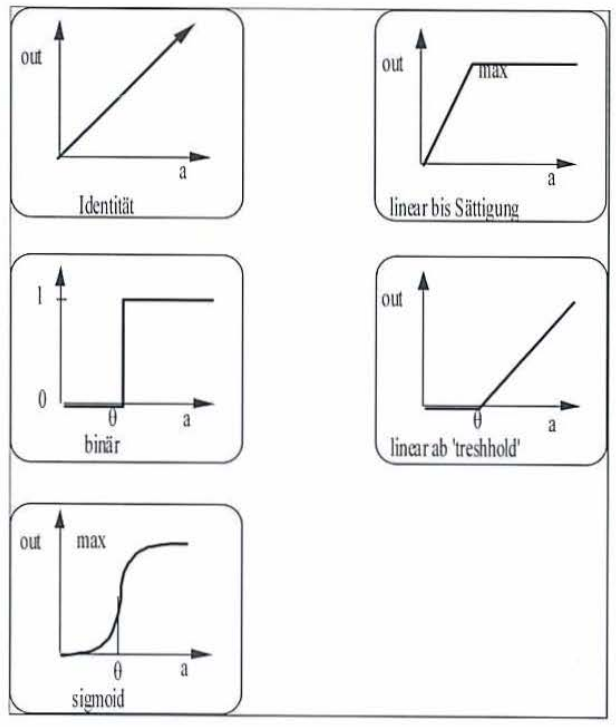
\includegraphics[width=\linewidth]{figures/ch01_Ausgabefunktion.png}
	\caption{Häufig verwendete Ausgabefunktionen}
	\label{fig:ausgabefunktionen}
\end{figure}

\subsection{Verbindungsnetzwerke}
Üblicherweise wird das Verbindungsnetzwerk der Zellen in
einer Matrixschreibweise angegeben: $w_{ij}$ ist eine Verbindung von Zelle $i$ nach Zelle $j$. Für die Verbindungsmatrix $\textbf{W} = [w_{ij}]$ gilt dann: ein Eintrag in der Matrix $\textbf{W}$ mit
\begin{itemize}
\item $w_{ij} = 0$ gibt an, daß keine Verbindung zwischen $i$ und $j$ existiert,
\item $w_{ij} < 0$ gibt an, daß Neuron $i$ seinen Nachfolger $j$ durch ein Gewicht der
Stärke $|w_{ij}|$ hemmt,
\item $w_{ij} > 0$ gibt an, daß Neuron $i$ seinen Nachfolger $j$ durch ein Gewicht der
Stärke $|w_{ij}|$ anregt.
\end{itemize}
%In der Implementierung in einem Software-Simulator wird häufig eine Speicherung der Verbindungsgewichte gewählt, bei der nur tatsächlich vorhandene Gewichte Speicherplatz benötigen, z.B. eine Zeigerstruktur, bei der jedes Neuron eine verkettete Liste aller Eingangsgewichte besitzt, von denen jedes wiederum einen Zeiger auf das Neuron besitzt, von dem die Verbindung ausgeht. Diese Art der Implementierung über sogenannte rückwärtsgerichtete Adjazenzlisten hat sich auf Workstations weitgehend durchgesetzt. Bei einer Realisierung als Matrix benötigt ein Netz mit n Neuronen nämlich immer Speicherplatz der Größe n^2 . Dies ist besonders für feedforward-Netze mit mehreren Ebenen eine große Verschwendung. 

Folgende Topologien neuronaler Netze kommen besonders häufig in Simulationen vor:
\begin{itemize}
\item \textbf{feedforward-Netze:} enthalten keine Zyklen
\item \textbf{feedback-Netze:} enthalten Zyklen (feedback)
\item \textbf{hierarchische Netze:} Gliederung in mehrere Ebenen
\end{itemize}

\subsection{Propagierungsregel}
gibt die Gesamteingabe aller Nachbarzellen an und hat bei sehr vielen Modellen die Form:\\
$net_j(t) = \sum_i o_i(t)w_{ij} = O(t)W_j$ (gewichtete Summe)\\
Dabei ist $O(t) = (o_1(t),...,o_n(t))$ ein Zeilenvektor, $W_j$ die $j$-te Spalte der Gewichtsmatrix $\textbf{W}$:\\
$Net(t) = O(t)W =  (o_1(t),...,o_n(t))\begin{pmatrix}
w_{11} & ... & w_{1m}\\
w_{n1} & ... & w_{nm}\\
\end{pmatrix}$

\subsection{Aktivierungsfunktion}
Berechnet einen Aktivierungszustand aus altem Zustand und Eingabewerten\\
$a_i(t+1) = f_{act}(a_i(t), net_i(t), \theta_i)$
\begin{itemize}
\item deterministische Aktivierungsfunktion $f$: Ergebnis eindeutig durch die Eingabe bestimmt
\item stochastische Aktivierungsfunktion $f$: Ergebnis durch eine Zufallsverteilung abhängig von der Eingabe bestimmt
\end{itemize}

\subsection{Lernregel}

Theoretisch mögliche Arten des Lernens:
\begin{itemize}
\item[1.]Entwicklung neuer Verbindungen
\item[2.]Löschen existierender Verbindungen
\item[3.]Modifikation der Stärke $w_{ij}$ von Verbindungen
\item[4.]Entwicklung neuer Zellen
\end{itemize}
1. und 2. kann durch 3. approximiert werden:\\
Neue Verbindung: $w_{ij} = 0 \rightarrow w_{ij} \neq 0$\\
Löschen: $w_{ij} \neq 0 \rightarrow w_{ij} = 0$
Aktuelle Lernverfahren arbeiten meist nur durch Modifikation der Verbindungen.
Tabelle \ref{tab:lernregeln} zeigt wichtige Lernregeln.
\begin{table}
\centering
\begin{tabular}{|l|}
	\hline
	Hebb'sche Lernregel: \\
	\hline
	Delta-Regel (Widrow-Hoff-Regel):\\
	\hline
	Grossberg's Regel:\\
	\hline
	Backpropagation (verallgem. Delta-Regel):\\
	\hline
\end{tabular}
\caption{Wichtige Lernregeln}
\label{tab:lernregeln}
\end{table}

\section*{Komponenten neuronaler Modelle}
% K
% Was es so für neuronale Modelle gibt